\documentclass[10pt]{article}
\usepackage[a4paper,margin=18mm]{geometry}
\usepackage[T1]{fontenc}\usepackage{lmodern}
\usepackage{amsmath,amssymb,booktabs,array,enumitem}
\usepackage{tikz}\usetikzlibrary{shapes.gates.logic.US,positioning,arrows.meta}
\usepackage[hidelinks]{hyperref}
\setlength{\parindent}{0pt}\setlength{\parskip}{4pt}\setlength{\emergencystretch}{2em}
\newcommand{\mos}[4]{\begin{scope}[shift={(#1,#2)}]
\draw(0,.24)--(0,-.24);\draw(0,.2)--(.25,.2)--(.25,.5);\draw(0,-.2)--(.25,-.2)--(.25,-.5);
\draw(-.16,.23)--(-.16,-.23);
\ifnum#4=1\draw(-.26,0)circle(.06);\draw(-.75,0)--(-.32,0);\else\draw(-.75,0)--(-.16,0);\fi
\node[anchor=east,font=\scriptsize]at(-.76,0){$#3$};\end{scope}}
\newcommand{\gnd}[2]{\draw(#1,#2)--(#1,{#2-.12});\draw({#1-.17},{#2-.12})--({#1+.17},{#2-.12});\draw({#1-.11},{#2-.2})--({#1+.11},{#2-.2});}
\newcommand{\rail}[3]{\draw(#1,#2)--(#1,{#2+.14});\node[above,font=\scriptsize]at(#1,{#2+.14}){$#3$};}
\begin{document}
\begin{center}{\Large 2008 Final: Independently Derived and Corrected Solutions}\end{center}
\textbf{Coverage and provenance.} All Q1--Q8 are complete, with printed weights totaling 115\%. The original footer explicitly says Fall 2008. \texttt{answer.pdf} and \texttt{final-answer.pdf} are byte-identical, and their correspondingly numbered photos are duplicate pairs: they form \emph{one} student-answer set, not two independent references. Both full answer pages were read after original-first derivation. Student identities, grades and unrelated handwritten marginal notes are not reproduced.

\textbf{Models.} Use the source's capacitance/leakage numbers, symbolic long-channel threshold-onset currents for Q6, and an ON-resistor model for the ratioed keeper in Q8. Bodies connect to the ordinary rails. Numeric parameters missing from a question remain symbolic; a parameter local to Q4 is not carried into Q6. Diagram symbols and repeated named terminals specify complete connectivity. No process-model simulation or DRC result is claimed.

\section*{Question 1: CMOS design, switching energy and logic}
\begin{enumerate}[label=(\alph*)]
\item Reduce shared package/supply return inductance using additional short parallel VDD/GND connections; reduce simultaneous $di/dt$ using controlled-slew or staged output drivers. $\Delta V\simeq L\,di/dt$ explains both. Local decoupling is another useful method. The student's multiple-pin idea is retained; ``avoid corners'' is not a universal substitute for designing a short, low-inductance current path.
\item Define specifications and logic; create/simulate the transistor schematic and size devices; draw layout; run DRC and LVS; extract parasitic R/C; perform post-layout simulation and iterate until signoff. The student's pre-simulation--layout--DRC/LVS--post-simulation sequence is useful, but add specification/schematic sizing and the parasitic-extraction step. The printed design flow is full-custom, so this concerns transistor/cell layout rather than merely placing predesigned cells.
\item From $P_{sw}=\alpha C V_{dd}^2f$, reduce unnecessary switching activity (clock gating, balanced arrivals/hazard reduction) and reduce switched capacitance (unnecessary buffers, wire load or oversized devices). Lower $V_{dd}$ is another method if timing/noise constraints permit it. The student's $\alpha,C,V_{dd}$ observations are retained with concrete examples.
\item With ideal capacitive load $C_L$, a 0-to-$V_{dd}$ output transition draws $Q=C_LV_{dd}$ and energy $E_{supply}=C_LV_{dd}^2$ from VDD. Half, $C_LV_{dd}^2/2$, is stored in the capacitor and half dissipates in the charging pMOS path. The falling transition draws no ideal charging energy from VDD; the stored half dissipates in the nMOS discharge path. A complete charge/discharge cycle dissipates $C_LV_{dd}^2$. Short-circuit/leakage and internal capacitances add energy in a real inverter. This missing student subanswer is completed; neither a single charging edge's supply energy nor a whole cycle is just $C_LV_{dd}^2/2$.
\item Charge sharing with initially low internal nodes and unsafe direct cascading of plain same-phase dynamic gates are two major problems. Leakage-induced loss of retained charge is another valid issue. Retain the student's first two points with the phase qualification.
\item Basic CMOS domino produces noninverting buffered functions, and evaluation inputs must remain stable or make the allowed nondecreasing transition for n-domino. Its per-stage output inverter is also an overhead/constraint, as the student notes. Arbitrary falling inputs or raw same-phase dynamic output cascades are unsafe.
\item Core-limited die size is determined by the logic/core area. Pad-limited die size is determined by IO pad count/pitch and perimeter even if a smaller core would suffice. These definitions complete the student's unlabelled sketches.
\end{enumerate}

\newpage\section*{Question 2: Complete complemented-function implementations}
Preserve the full overbar: $h=A(B+C)+DE$ and
\[\boxed{f=\bar h=(\bar A+\bar B\bar C)(\bar D+\bar E).}\]
Here diagram output F denotes f. Five explicit CMOS inverters generate $\bar A,\bar B,\bar C,\bar D,\bar E$ when only the original inputs are supplied (p/n gates at each original input, common complement drain and rail sources).

\textbf{Domino.} The nMOS PDN implements \emph{f}, with $\bar A$ parallel to series $\bar B$--$\bar C$, then in series with parallel $\bar D$/$\bar E$. Its dynamic node Z precharges high and discharges when f=1; the output CMOS inverter gives f. The five data nMOS plus precharge/footer and two-device output inverter give 9 core MOS, or 19 with the five complement generators. Their inputs must settle before evaluation or obey the required monotone protocol.
\begin{center}\begin{tikzpicture}[x=.92cm,y=.92cm,font=\scriptsize]
\mos{0.0}{0.0}{\bar A}{0}
\node[right]at(0.43,0.0){$\mathrm{NAbar}$};
\node[above]at(0.25,0.52){$Z$};
\node[below]at(0.25,-0.52){$g1$};
\mos{3.9}{0.0}{\bar B}{0}
\node[right]at(4.33,0.0){$\mathrm{NBbar}$};
\node[above]at(4.15,0.52){$Z$};
\node[below]at(4.15,-0.52){$g2$};
\mos{7.8}{0.0}{\bar C}{0}
\node[right]at(8.23,0.0){$\mathrm{NCbar}$};
\node[above]at(8.05,0.52){$g2$};
\node[below]at(8.05,-0.52){$g1$};
\mos{11.7}{0.0}{\bar D}{0}
\node[right]at(12.129999999999999,0.0){$\mathrm{NDbar}$};
\node[above]at(11.95,0.52){$g1$};
\node[below]at(11.95,-0.52){$foot$};
\mos{0.0}{-2.2}{\bar E}{0}
\node[right]at(0.43,-2.2){$\mathrm{NEbar}$};
\node[above]at(0.25,-1.6800000000000002){$g1$};
\node[below]at(0.25,-2.72){$foot$};
\mos{3.9}{-2.2}{\phi}{1}
\node[right]at(4.33,-2.2){$\mathrm{Ppre}$};
\node[above]at(4.15,-1.6800000000000002){$V_{DD}$};
\node[below]at(4.15,-2.72){$Z$};
\mos{7.8}{-2.2}{\phi}{0}
\node[right]at(8.23,-2.2){$\mathrm{Nfoot}$};
\node[above]at(8.05,-1.6800000000000002){$foot$};
\node[below]at(8.05,-2.72){$V_{SS}$};
\mos{11.7}{-2.2}{Z}{1}
\node[right]at(12.129999999999999,-2.2){$\mathrm{Pout}$};
\node[above]at(11.95,-1.6800000000000002){$V_{DD}$};
\node[below]at(11.95,-2.72){$F$};
\mos{0.0}{-4.4}{Z}{0}
\node[right]at(0.43,-4.4){$\mathrm{Nout}$};
\node[above]at(0.25,-3.8800000000000003){$F$};
\node[below]at(0.25,-4.92){$V_{SS}$};
\end{tikzpicture}\end{center}
Equal named channel ends connect the series/parallel paths. In particular foot connects only through the clock footer to ground. Using the h pull-down and then a domino inverter would yield h, which is the wrong output polarity.

\newpage\textbf{Q2, fully differential.} Use an f-side nMOS pull-down h, and a $\bar f$-side nMOS pull-down f. Cross-coupled pMOS loads have sources at VDD, drains at their output and gates at the opposite output. The core has ten nMOS and two pMOS (12 total), or 22 with complements.
\begin{center}\begin{tikzpicture}[x=.92cm,y=.92cm,font=\scriptsize]
\mos{0.0}{0.0}{A}{0}
\node[right]at(0.43,0.0){$\mathrm{NA}$};
\node[above]at(0.25,0.52){$F$};
\node[below]at(0.25,-0.52){$bc$};
\mos{3.9}{0.0}{B}{0}
\node[right]at(4.33,0.0){$\mathrm{NB}$};
\node[above]at(4.15,0.52){$bc$};
\node[below]at(4.15,-0.52){$V_{SS}$};
\mos{7.8}{0.0}{C}{0}
\node[right]at(8.23,0.0){$\mathrm{NC}$};
\node[above]at(8.05,0.52){$bc$};
\node[below]at(8.05,-0.52){$V_{SS}$};
\mos{11.7}{0.0}{D}{0}
\node[right]at(12.129999999999999,0.0){$\mathrm{ND}$};
\node[above]at(11.95,0.52){$F$};
\node[below]at(11.95,-0.52){$de$};
\mos{0.0}{-2.2}{E}{0}
\node[right]at(0.43,-2.2){$\mathrm{NE}$};
\node[above]at(0.25,-1.6800000000000002){$de$};
\node[below]at(0.25,-2.72){$V_{SS}$};
\mos{3.9}{-2.2}{\bar A}{0}
\node[right]at(4.33,-2.2){$\mathrm{NAbar}$};
\node[above]at(4.15,-1.6800000000000002){$\bar F$};
\node[below]at(4.15,-2.72){$g1$};
\mos{7.8}{-2.2}{\bar B}{0}
\node[right]at(8.23,-2.2){$\mathrm{NBbar}$};
\node[above]at(8.05,-1.6800000000000002){$\bar F$};
\node[below]at(8.05,-2.72){$g2$};
\mos{11.7}{-2.2}{\bar C}{0}
\node[right]at(12.129999999999999,-2.2){$\mathrm{NCbar}$};
\node[above]at(11.95,-1.6800000000000002){$g2$};
\node[below]at(11.95,-2.72){$g1$};
\mos{0.0}{-4.4}{\bar D}{0}
\node[right]at(0.43,-4.4){$\mathrm{NDbar}$};
\node[above]at(0.25,-3.8800000000000003){$g1$};
\node[below]at(0.25,-4.92){$V_{SS}$};
\mos{3.9}{-4.4}{\bar E}{0}
\node[right]at(4.33,-4.4){$\mathrm{NEbar}$};
\node[above]at(4.15,-3.8800000000000003){$g1$};
\node[below]at(4.15,-4.92){$V_{SS}$};
\mos{7.8}{-4.4}{\bar F}{1}
\node[right]at(8.23,-4.4){$\mathrm{PF}$};
\node[above]at(8.05,-3.8800000000000003){$V_{DD}$};
\node[below]at(8.05,-4.92){$F$};
\mos{11.7}{-4.4}{F}{1}
\node[right]at(12.129999999999999,-4.4){$\mathrm{PFbar}$};
\node[above]at(11.95,-3.8800000000000003){$V_{DD}$};
\node[below]at(11.95,-4.92){$\bar F$};
\end{tikzpicture}\end{center}
\textbf{Q2, static CMOS.} The h pull-down has A in series with parallel B/C, in parallel with series D/E. Its dual pMOS pull-up has parallel A versus series B/C, in series with parallel D/E; original inputs drive the p gates. It has five pMOS plus five nMOS, 10 total, and produces f without input complement generators.
\begin{center}\begin{tikzpicture}[x=.92cm,y=.92cm,font=\scriptsize]
\mos{0.0}{0.0}{A}{0}
\node[right]at(0.43,0.0){$\mathrm{NA}$};
\node[above]at(0.25,0.52){$F$};
\node[below]at(0.25,-0.52){$bc$};
\mos{3.9}{0.0}{B}{0}
\node[right]at(4.33,0.0){$\mathrm{NB}$};
\node[above]at(4.15,0.52){$bc$};
\node[below]at(4.15,-0.52){$V_{SS}$};
\mos{7.8}{0.0}{C}{0}
\node[right]at(8.23,0.0){$\mathrm{NC}$};
\node[above]at(8.05,0.52){$bc$};
\node[below]at(8.05,-0.52){$V_{SS}$};
\mos{11.7}{0.0}{D}{0}
\node[right]at(12.129999999999999,0.0){$\mathrm{ND}$};
\node[above]at(11.95,0.52){$F$};
\node[below]at(11.95,-0.52){$de$};
\mos{0.0}{-2.2}{E}{0}
\node[right]at(0.43,-2.2){$\mathrm{NE}$};
\node[above]at(0.25,-1.6800000000000002){$de$};
\node[below]at(0.25,-2.72){$V_{SS}$};
\mos{3.9}{-2.2}{A}{1}
\node[right]at(4.33,-2.2){$\mathrm{PA}$};
\node[above]at(4.15,-1.6800000000000002){$V_{DD}$};
\node[below]at(4.15,-2.72){$p1$};
\mos{7.8}{-2.2}{B}{1}
\node[right]at(8.23,-2.2){$\mathrm{PB}$};
\node[above]at(8.05,-1.6800000000000002){$V_{DD}$};
\node[below]at(8.05,-2.72){$p2$};
\mos{11.7}{-2.2}{C}{1}
\node[right]at(12.129999999999999,-2.2){$\mathrm{PC}$};
\node[above]at(11.95,-1.6800000000000002){$p2$};
\node[below]at(11.95,-2.72){$p1$};
\mos{0.0}{-4.4}{D}{1}
\node[right]at(0.43,-4.4){$\mathrm{PD}$};
\node[above]at(0.25,-3.8800000000000003){$p1$};
\node[below]at(0.25,-4.92){$F$};
\mos{3.9}{-4.4}{E}{1}
\node[right]at(4.33,-4.4){$\mathrm{PE}$};
\node[above]at(4.15,-3.8800000000000003){$p1$};
\node[below]at(4.15,-4.92){$F$};
\end{tikzpicture}\end{center}
\textbf{Student comparison.} Retain the Boolean complement identity, cross-coupled differential concept and dual static topology. The domino sketch lacks its complete clock/reset/output-inverter implementation and complementary-input generation. The diagrams/netlists here restore all support devices and preserve the requested f polarity. Thirty-two input truths, sixty-four domino phases and one hundred twenty-eight differential candidate states are independently checked.

\newpage\section*{Question 3: Positive-edge dynamic CMOS register}
Read the printed clock bubbles, excluding pen crosses: the \emph{first two} clock-controlled middle devices are pMOS; the last two are nMOS. The four three-device stages contain twelve MOS.

When $\phi=0$, the first two p-clocked stages evaluate $A=\bar I$ and $B=\bar A=I$. The slave's two n-clocked stages cannot discharge through their clock devices, so O holds its previous sample. C can rise when B=0, but that only turns off its following pull-up; it cannot cause O to discharge through the disabled clock path.

At the \textbf{rising edge} $\phi:0\to1$, the master stops tracking and B retains the pre-edge I. The two slave stages evaluate $C=\bar B$ and $O=\bar C=B$. During the high phase, a new input can pull A downward, but cannot charge it; B can be forced low only by A=1, which already corresponds to a retained B=0. Therefore B and O keep the sample despite later I changes. The circuit is a
\[\boxed{\text{positive-edge, noninverting dynamic register}.}\]
\begin{center}\begin{tikzpicture}[scale=.9,font=\small]
\foreach \x in {0,3,6,9}{\rail{\x+.25}{4}{V_{DD}}\gnd{\x+.25}{.2}}
\mos{0}{3.5}{}{1}\mos{0}{2.1}{\phi}{1}\mos{0}{.7}{}{0}\draw(.25,3)--(.25,2.6);\draw(.25,1.6)--(.25,1.2);
\mos{3}{3.5}{}{1}\mos{3}{2.1}{\phi}{1}\mos{3}{.7}{}{0}\draw(3.25,3)--(3.25,2.6);\draw(3.25,1.6)--(3.25,1.2);
\mos{6}{3.5}{}{1}\mos{6}{2.1}{\phi}{0}\mos{6}{.7}{}{0}\draw(6.25,3)--(6.25,2.6);\draw(6.25,1.6)--(6.25,1.2);
\mos{9}{3.5}{}{1}\mos{9}{2.1}{\phi}{0}\mos{9}{.7}{}{0}\draw(9.25,3)--(9.25,2.6);\draw(9.25,1.6)--(9.25,1.2);
\draw(-.75,3.5)--(-1.3,3.5)--(-1.3,.7)--(-.75,.7);\draw(-1.3,2.8)--(-2,2.8)node[left]{$I$};\draw(.25,1.4)--(1.7,1.4)--(1.7,3.5)--(2.25,3.5);\draw(1.7,1.4)--(1.7,.7)--(2.25,.7);\node[above]at(.8,1.4){$A$};\fill(1.7,1.4)circle(1.5pt);
\draw(3.25,1.4)--(4.7,1.4)--(4.7,3.5)--(5.25,3.5);\draw(4.7,1.4)--(4.7,.7)--(5.25,.7);\node[above]at(3.9,1.4){$B$};\fill(4.7,1.4)circle(1.5pt);
\draw(6.25,2.8)--(7.7,2.8)--(7.7,3.5)--(8.25,3.5);\draw(7.7,2.8)--(7.7,.7)--(8.25,.7);\node[below]at(6.9,2.8){$C$};\fill(7.7,2.8)circle(1.5pt);\draw(9.25,2.8)--(11,2.8)node[right]{$O$};
\end{tikzpicture}\\Figure 1: A dynamic CMOS register circuit. All four three-device stages and the two first-stage clock-controlled pMOS bubbles are retained.\end{center}
\begin{center}\begin{tabular}{c|lll}\toprule
Phase&Master A/B&Slave C&Output O\\\midrule
$\phi=0$&$A=\bar I,\ B=I$&May rise for B=0, otherwise retains&Old sample held\\
$0\to1$&B captures I&$C=\bar B$&$O=B$ after settling\\
$\phi=1$&B holds despite input changes&$C=\bar B$&Captured sample held\\\bottomrule
\end{tabular}\end{center}
Held dynamic nodes rely on charge and need a valid phase sequence, setup/settling time and refresh against leakage. No numerical retention limit is given for this question. A floating power-up node is not assigned a fabricated initial value. The supplied student pages have no complete usable Q3 operation answer; the eight source-derived phase histories complete it. This circuit's clock polarity is the reverse of the 2009 final's superficially similar register.

\newpage\section*{Question 4: NP full-adder retention and duty dependence}
\textbf{(a)} This is NP-domino logic: an n-dynamic carry stage precharges high and can fall during evaluation; a p-dynamic sum stage resets low and can rise. Both output inverters are \emph{static}. With $M=A_nB_n+C_n(A_n+B_n)$, the first dynamic output is $z=\bar C_{n+1}=\bar M$, and carry $C_{n+1}=M$. The p network conducts for
\[(\bar A_n+\bar B_n+\bar C_n)(\bar z+\bar A_n\bar B_n\bar C_n),\]
giving $w=\bar S_n$ even parity; the output inverter gives $S_n=A_n\oplus B_n\oplus C_n$. During $\phi=0$, z=1/w=0; during evaluation $\phi=1$, z may fall and w may rise, with data stable. The source has 20 MOS, not clocked output-inverter variants from other years.

\textbf{(b)} Count every connected terminal using the full graph, with source $C_d=0.2\,fF$ and $C_g=1\,fF$ for \emph{each} p/n device:
\begin{center}\begin{tabular}{l|ccr}\toprule
Node&Diffusion caps&Gate caps&Total\\\midrule
$z=\bar C_{n+1}$&3: precharge p, top A n, top C n&3: both carry INV gates and pz&$3.6\,fF$\\
$w=\bar S_n$&3: reset n, direct pz, last series pC&2: both sum INV gates&$2.6\,fF$\\\bottomrule
\end{tabular}\end{center}
Output-inverter drain capacitances belong to the buffered outputs, rather than z/w. The gate capacitance of clock devices belongs to the clock. No unprinted 2:1 p/n gate-cap factor is applied.

Take the specified 1 nA at each node as the adverse net leakage magnitude. Floating high z can decay from 1.8 V toward the 1 V inverter trip; floating low w can rise from zero toward that trip. Their retention limits differ:
\[t_z=\frac{3.6\,fF(1.8-1)\,V}{1\,nA}=2.88\,\mu s,\qquad
t_w=\frac{2.6\,fF(1-0)\,V}{1\,nA}=2.60\,\mu s.\]
\[\boxed{t_{evaluation/hold}<2.60\,\mu s.}\]
Equality leaves a node at the switching point, with no logic margin. If D is the \emph{evaluation duty fraction}, the printed question does not specify D, so
\[\boxed{\frac{D}{f}<2.60\,\mu s\quad\Longleftrightarrow\quad f>384.615D\,kHz.}\]
An explicitly assumed 50\% clock has boundary 192.308 kHz. A conservative whole-period retention allocation has boundary 384.615 kHz. Neither is a uniquely determined duty-independent frequency from the original; the primary result is the hold bound and duty formula. Precharge actively restores both nodes; leakage is one total current per node, not one per diffusion terminal.

\textbf{Student comparison.} Retain its corrected $3C_d+3C_g$ and $3C_d+2C_g$ counts. Complete the separate high/low voltage margins, critical-node comparison and duty-dependent frequency. Applying the high-node margin $V_{dd}-V_M$ to the low sum node would be incorrect. The source constant-leakage model is an analytical bound, not characterized process leakage.

\newpage\section*{Question 5: 100 MHz setup, missing hold parameter}
At 100 MHz, $T=10\,ns$. The source gives $t_{pcq}=1\,ns$ and $t_{setup}=1.5\,ns$. Setup requires
\[T\ge t_{pcq}+t_{pd}+t_{setup}\quad\Longrightarrow\quad
\boxed{t_{pd,comb}\le7.5\,ns.}\]
The hold time is 1 ns, so $t_{ccq}+t_{cd,comb}\ge1\,ns$. But the source omits clock-to-Q \emph{contamination} delay; it is not the given propagation delay. Thus
\[\boxed{t_{cd,comb}\ge\max(0,1\,ns-t_{ccq}),}\]
with no unique numeric lower bound inferred. A conservative choice valid for any nonnegative $t_{ccq}$ is $t_{cd,comb}\ge1\,ns$, explicitly a design bound rather than an inferred source value. The common source clock has no specified skew. Increasing the period does not repair a hold violation.
\begin{center}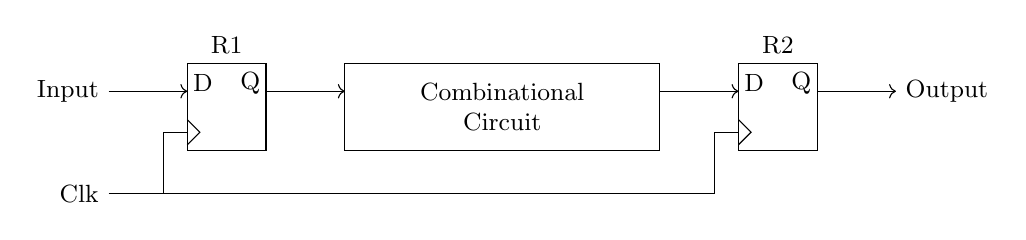
\begin{tikzpicture}[font=\small]
\foreach \x/\name in {0/R1,7/R2}{\draw(\x,-.45)rectangle(\x+1,.65);\node at(\x+.2,.4){D};\node at(\x+.8,.4){Q};\draw(\x,-.38)--(\x+.16,-.22)--(\x,-.06);\node[above]at(\x+.5,.65){\name};\draw(\x-.3,-1)--(\x-.3,-.22)--(\x,-.22);}
\draw(2,.65)rectangle(6,-.45);\node[align=center]at(4,.1){Combinational\\Circuit};\draw[->](-1,.3)--(0,.3);\node[left]at(-1,.3){Input};\draw[->](1,.3)--(2,.3);\draw[->](6,.3)--(7,.3);\draw[->](8,.3)--(9,.3)node[right]{Output};\draw(-1,-1)--(6.7,-1);\node[left]at(-1,-1){Clk};
\end{tikzpicture}\\Figure 3: A pipelined circuit.\end{center}
\textbf{Student comparison.} Retain the correct setup/hold inequalities, finish the 7.5 ns setup arithmetic and state the missing $t_{ccq}$. Do not silently substitute 1 ns propagation delay into the hold equation.

\section*{Question 6: Schmitt sizes are a threshold-dependent family}
The source gives $V_{T+}=0.7V_{dd}$, $V_{T-}=0.3V_{dd}$, reference $(W/L)_{N1}=4$, and $(W/L)_{P1}=6$. It gives neither $V_{tn}$ nor $|V_{tp}|$, nor the feedback-device channel lengths. The 1.8 V/1 V values in Q4 are \emph{local} premises and do not fill these gaps.

In the ordinary fixed-threshold square-law onset approximation, before a rising trip $V_{out}\simeq V_{dd}$. N2 reaches onset at internal node $u=V_{T+}-V_{tn}$. N1 has overdrive and drain voltage $0.7V_{dd}-V_{tn}$, at its saturation boundary. Feedback N3 has gate/drain at VDD and source u; its saturated overdrive is $0.3V_{dd}$. Current balance gives
\[\frac12\beta_{N1}(0.7V_{dd}-V_{tn})^2=\frac12\beta_{N3}(0.3V_{dd})^2,\]
\[\boxed{(W/L)_{N3}=4\left(\frac{0.7V_{dd}-V_{tn}}{0.3V_{dd}}\right)^2.}\]
Before the falling trip $V_{out}\simeq0$. P2 begins conducting at internal p node $v=V_{T-}+|V_{tp}|$. P1 is at the saturation boundary with overdrive $0.7V_{dd}-|V_{tp}|$; P3 is saturated with overdrive $0.3V_{dd}$. Hence
\[\boxed{(W/L)_{P3}=6\left(\frac{0.7V_{dd}-|V_{tp}|}{0.3V_{dd}}\right)^2.}\]
The model requires positive overdrives, $V_{tn}<0.7V_{dd}$ and $|V_{tp}|<0.7V_{dd}$. If feedback lengths are \emph{chosen} as 0.5 $\mu m$, widths are $2\,\mu m$ and $3\,\mu m$ times the corresponding squared ratios. No unique numerical widths follow without the omitted thresholds. This fixed-threshold onset model excludes unprovided body effect/channel-length modulation and is not a complete VTC simulation.

\textbf{Student comparison.} The first internal-node equation $u=V_{T+}-V_{tn}$ is useful. Its later constant-resistance division treats N2 as fully ON at onset and drops the threshold offset; that does not determine valid scalar dimensions. Replace it by the symbolic MOS-current family. The saved normalized threshold samples verify algebra only and are explicitly hypothetical, not adopted physical parameters.

\newpage\section*{Question 7: Literal source layouts}
\textbf{(a)} The first source layout has \emph{four} crossings per row, eight MOS: two TGs and two inverters. A faithful native-pixel check resolves the apparent overlap at its midpoint. In the original 1648-by-2338 TIFF, rectangle x=455--464, y=1690--1708 contains 190 completely white pixels separating the left Y metal stripe from the independent right clock/contact stripe. The latter connects first n gate C to second p gate C, while the opposite poly route connects first p $\bar C$ to second n $\bar C$. Thus the second gate is a split clock TG, not an inverter with input Y. The original pixel evidence is saved separately; no scan pixel was altered.
Introduce internal nets u and v:
\begin{center}\begin{tabular}{c|ccc|ccc}\toprule
Column&p left&p right&p gate&n left&n right&n gate\\\midrule
1&Y&u&$\bar C$&Y&u&C\\2&u&v&C&u&v&$\bar C$\\
3&v&$V_{DD}$&X&v&$V_{SS}$&X\\4&$V_{DD}$&X&u&$V_{SS}$&X&u\\\bottomrule
\end{tabular}\end{center}
\begin{center}\begin{tikzpicture}[x=.92cm,y=.92cm,font=\scriptsize]
\mos{0.0}{0.0}{\bar C}{1}
\node[right]at(0.43,0.0){$\mathrm{P1}$};
\node[above]at(0.25,0.52){$Y$};
\node[below]at(0.25,-0.52){$u$};
\mos{3.9}{0.0}{C}{0}
\node[right]at(4.33,0.0){$\mathrm{N1}$};
\node[above]at(4.15,0.52){$Y$};
\node[below]at(4.15,-0.52){$u$};
\mos{7.8}{0.0}{C}{1}
\node[right]at(8.23,0.0){$\mathrm{P2}$};
\node[above]at(8.05,0.52){$u$};
\node[below]at(8.05,-0.52){$v$};
\mos{11.7}{0.0}{\bar C}{0}
\node[right]at(12.129999999999999,0.0){$\mathrm{N2}$};
\node[above]at(11.95,0.52){$u$};
\node[below]at(11.95,-0.52){$v$};
\mos{0.0}{-2.2}{X}{1}
\node[right]at(0.43,-2.2){$\mathrm{P3}$};
\node[above]at(0.25,-1.6800000000000002){$v$};
\node[below]at(0.25,-2.72){$V_{DD}$};
\mos{3.9}{-2.2}{X}{0}
\node[right]at(4.33,-2.2){$\mathrm{N3}$};
\node[above]at(4.15,-1.6800000000000002){$v$};
\node[below]at(4.15,-2.72){$V_{SS}$};
\mos{7.8}{-2.2}{u}{1}
\node[right]at(8.23,-2.2){$\mathrm{P4}$};
\node[above]at(8.05,-1.6800000000000002){$V_{DD}$};
\node[below]at(8.05,-2.72){$X$};
\mos{11.7}{-2.2}{u}{0}
\node[right]at(12.129999999999999,-2.2){$\mathrm{N4}$};
\node[above]at(11.95,-1.6800000000000002){$V_{SS}$};
\node[below]at(11.95,-2.72){$X$};
\end{tikzpicture}\end{center}
For C=1 the input Y--u TG is ON and the u--v feedback TG is OFF; the u-to-X inverter gives $X=\bar Y$. For C=0 the input TG is OFF and feedback TG closes the two-inverter loop, retaining either state. It is a positive-level \emph{inverting} static latch. No outer input inverter or self-connected last pair from another year's larger layout is inserted.

\textbf{(b)} The second source layout has six crossings per row, twelve MOS. Its central pMOS are \emph{parallel}, with alternating VDD/Z contact intervals, and its central nMOS are \emph{series}, with no intermediate contact straps. Columns 1, 2 and 6 have p gates at VDD and n gates at VSS; these six OFF devices and their floating stubs are retained.
\[\boxed{Z=\overline{abc}\quad\text{(NAND3 functional core; 12 physical MOS).}}\]
\begin{center}\begin{tikzpicture}[x=.92cm,y=.92cm,font=\scriptsize]
\mos{0.0}{0.0}{V_{DD}}{1}
\node[right]at(0.43,0.0){$\mathrm{P1}$};
\node[above]at(0.25,0.52){$p0$};
\node[below]at(0.25,-0.52){$p1$};
\mos{3.9}{0.0}{V_{SS}}{0}
\node[right]at(4.33,0.0){$\mathrm{N1}$};
\node[above]at(4.15,0.52){$n0$};
\node[below]at(4.15,-0.52){$n1$};
\mos{7.8}{0.0}{V_{DD}}{1}
\node[right]at(8.23,0.0){$\mathrm{P2}$};
\node[above]at(8.05,0.52){$p1$};
\node[below]at(8.05,-0.52){$V_{DD}$};
\mos{11.7}{0.0}{V_{SS}}{0}
\node[right]at(12.129999999999999,0.0){$\mathrm{N2}$};
\node[above]at(11.95,0.52){$n1$};
\node[below]at(11.95,-0.52){$V_{SS}$};
\mos{0.0}{-2.2}{a}{1}
\node[right]at(0.43,-2.2){$\mathrm{P3}$};
\node[above]at(0.25,-1.6800000000000002){$V_{DD}$};
\node[below]at(0.25,-2.72){$Z$};
\mos{3.9}{-2.2}{a}{0}
\node[right]at(4.33,-2.2){$\mathrm{N3}$};
\node[above]at(4.15,-1.6800000000000002){$V_{SS}$};
\node[below]at(4.15,-2.72){$n3$};
\mos{7.8}{-2.2}{b}{1}
\node[right]at(8.23,-2.2){$\mathrm{P4}$};
\node[above]at(8.05,-1.6800000000000002){$Z$};
\node[below]at(8.05,-2.72){$V_{DD}$};
\mos{11.7}{-2.2}{b}{0}
\node[right]at(12.129999999999999,-2.2){$\mathrm{N4}$};
\node[above]at(11.95,-1.6800000000000002){$n3$};
\node[below]at(11.95,-2.72){$n4$};
\mos{0.0}{-4.4}{c}{1}
\node[right]at(0.43,-4.4){$\mathrm{P5}$};
\node[above]at(0.25,-3.8800000000000003){$V_{DD}$};
\node[below]at(0.25,-4.92){$Z$};
\mos{3.9}{-4.4}{c}{0}
\node[right]at(4.33,-4.4){$\mathrm{N5}$};
\node[above]at(4.15,-3.8800000000000003){$n4$};
\node[below]at(4.15,-4.92){$Z$};
\mos{7.8}{-4.4}{V_{DD}}{1}
\node[right]at(8.23,-4.4){$\mathrm{P6}$};
\node[above]at(8.05,-3.8800000000000003){$Z$};
\node[below]at(8.05,-4.92){$p6$};
\mos{11.7}{-4.4}{V_{SS}}{0}
\node[right]at(12.129999999999999,-4.4){$\mathrm{N6}$};
\node[above]at(11.95,-3.8800000000000003){$Z$};
\node[below]at(11.95,-4.92){$n6$};
\end{tikzpicture}\end{center}
The p interval connections are $p_0,p_1,V_{DD},Z,V_{DD},Z,p_6$ left to right; the n intervals are $n_0,n_1,V_{SS},n_3,n_4,Z,n_6$. Equal named channel ends in the schematics are connected. The source is not the NOR3 layout from 2012/2013, so that answer is not reused by visual resemblance. Eight input truths confirm exactly one functional rail path for each abc state.

\textbf{Student comparison.} The supplied answer does not provide a complete transistor-level extraction for either layout. Its unlabelled pass/clock sketches are insufficient to validate the source contacts; the literal eight- and twelve-MOS netlists above complete the requested schematics.

\newpage\section*{Question 8: Weak keeper sizes and falling-edge register}
\textbf{(a)} The upstream p-network is series A/B in parallel with C, with each p $W/L=2$. The n-network is C in series with parallel A/B, each n $W/L=1$. Thus its output is $U=\overline{C(A+B)}$ (OAI21). The enabled TG has zero resistance/capacitance by the source premise and transfers U to Inv1 input s; Inv1 yields $Q=C(A+B)$ while CLK=1.

Let R be the ON resistance of a unit $W/L=1$ nMOS. From $\mu_n=2\mu_p$, a $W/L=2$ pMOS has the same R. Worst upstream high drive uses the A/B p series path, 2R; worst low drive uses C plus one A/B n device, 2R. Parallel alternatives are stronger.

For feedback inverter-2 p width ratio $w_p=(W/L)_{p2}$ and n ratio $w_n=(W/L)_{n2}$, resistances are $R_{pk}=2R/w_p$ and $R_{nk}=R/w_n$. Overwriting old s=1 needs the upstream 2R pull-down to cross the VDD/2 threshold despite its old p keeper:
\[\frac{V_s}{V_{dd}}=\frac{2R}{R_{pk}+2R}<\frac12\ \Longrightarrow\ R_{pk}>2R\ \Longrightarrow\ \boxed{0<w_p<1.}\]
Overwriting old s=0 needs the upstream 2R pull-up to cross upward against its n keeper:
\[\frac{V_s}{V_{dd}}=\frac{R_{nk}}{2R+R_{nk}}>\frac12\ \Longrightarrow\ R_{nk}>2R\ \Longrightarrow\ \boxed{0<w_n<0.5.}\]
Equality gives no write margin. This is a weak-keeper family, not a unique pair of sizes. A usual equal-strength choice $w_p=2w_n$, with $w_n<0.5$, satisfies both overwrite bounds; the source separately supplies the inverter switching voltage. No leakage/noise data gives a numerical lower bound on keeper strength. The saved checks enumerate all upstream parallel paths and two hundred overwrite-divider cases.

\textbf{(b)} Read the two mux labels rather than the faulty panel reference. The upper drawing selects D at CLK=0 and feedback at CLK=1, a low-level latch. The lower selects D at CLK=1 and feedback at CLK=0, a high-level latch. Both triangles are \emph{noninverting buffers}, with no output bubble.

Connect the \emph{lower/high-level} latch first as master and the \emph{upper/low-level} latch second as slave, sharing the same CLK. During CLK=1, master M follows D while Q holds. At $1\to0$, M captures D and the slave opens to deliver M. During CLK=0, later D changes cannot pass the closed master, so Q retains its sample. No clock inversion is needed because the source muxes already have complementary selections.
\begin{center}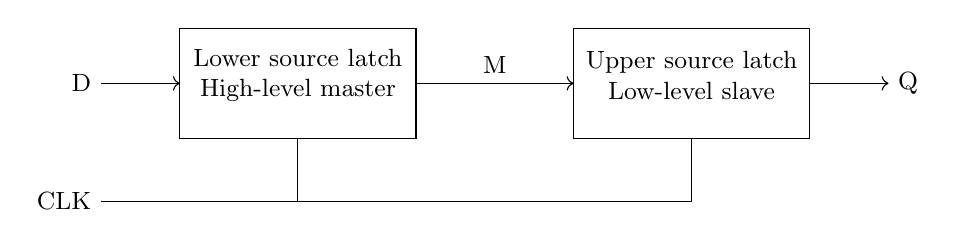
\begin{tikzpicture}[font=\small]
\draw(0,0)rectangle(3,1.4);\draw(5,0)rectangle(8,1.4);\node[align=center]at(1.5,.8){Lower source latch\\High-level master};\node[align=center]at(6.5,.8){Upper source latch\\Low-level slave};\draw[->](-1,.7)--(0,.7)node[pos=0,left]{D};\draw[->](3,.7)--(5,.7)node[midway,above]{M};\draw[->](8,.7)--(9,.7)node[right]{Q};\draw(-1,-.8)--(6.5,-.8)--(6.5,0);\draw(1.5,-.8)--(1.5,0);\node[left]at(-1,-.8){CLK};
\end{tikzpicture}\end{center}
\begin{center}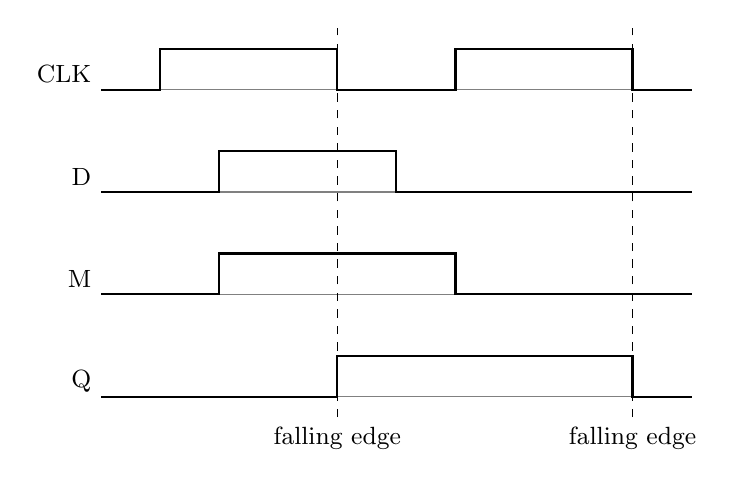
\begin{tikzpicture}[x=.75cm,y=.65cm,font=\small]
\foreach \y/\n in {6/CLK,4/D,2/M,0/Q}{\draw[gray](0,\y)--(10,\y);\node[left]at(0,\y+.3){\n};}
\draw[thick](0,6)--(1,6)--(1,6.8)--(4,6.8)--(4,6)--(6,6)--(6,6.8)--(9,6.8)--(9,6)--(10,6);
\draw[thick](0,4)--(2,4)--(2,4.8)--(5,4.8)--(5,4)--(10,4);
\draw[thick](0,2)--(2,2)--(2,2.8)--(6,2.8)--(6,2)--(10,2);
\draw[thick](0,0)--(4,0)--(4,.8)--(9,.8)--(9,0)--(10,0);
\draw[dashed](4,-.4)--(4,7.2);\draw[dashed](9,-.4)--(9,7.2);\node[below]at(4,-.4){falling edge};\node[below]at(9,-.4){falling edge};
\end{tikzpicture}\\Ideal sequencing only; no numerical latch delays are assigned. Q changes at falling edges and retains the sampled value when D changes during the low phase.\end{center}
The model assumes valid setup/settling and ideal phase sequencing; numerical delay/clock-overlap values are unprovided. Thirty-two two-cycle sequences independently verify noninverting Q updates only at falling edges. The original text's Figure 6(c) and repeated ``low-level'' caption are panel-label/description typos, not missing circuit premises. The student pages have no complete usable keeper-size or labelled mux/order/timing solution; these are derived from the actual source.

\section*{Verification and source comparison}
Run \texttt{python verify.py} to regenerate all saved CSV/JSON evidence. Checks cover Q2's thirty-two functions and full transistor graphs; Q3 positive-edge phase histories; Q4 full-adder truth, dynamic-node caps and duty-dependent retention; Q5 setup/conditional hold; Q6 symbolic onset currents/regions; Q7 all literal devices, latch states and NAND3 truths; and Q8 upstream resistances, keeper overwrite and falling-edge sequences. They are analytical proofs/checks, not simulation or DRC. Exact white-gap coordinates, anonymized comparison, question coverage, compiler results and all-page visual QA are recorded.

\begin{center}\begin{tabular}{lp{11.5cm}}\toprule
Question&Reproducible result and scope\\\midrule
Q2&32 input truths; 64 domino phases; 128 differential candidate states. Core/complete counts: domino 9/19, differential 12/22; static CMOS 10.\\
Q3&12 physical MOS; eight phase histories establish rising-edge noninverting capture and high-phase retention.\\
Q4&20 physical MOS; eight full-adder truths; connected-terminal caps $C_z=3.6\,fF$ and $C_w=2.6\,fF$; strict hold time below $2.60\,\mu s$. Clock duty remains symbolic.\\
Q5&Setup bound $t_{pd}\le7.5\,ns$; hold bound $t_{cd}\ge\max(0,1\,ns-t_{ccq})$. The omitted $t_{ccq}$ is not assigned.\\
Q6&Fourteen normalized threshold samples check current equality and onset regions in the symbolic sizing family; the samples are hypothetical algebraic checks.\\
Q7(a)&Eight physical MOS, two TGs and two inverters; 32 candidate states check transparent inversion and both closed-latch states. Native source gap: 190 white pixels.\\
Q7(b)&Twelve physical MOS including six OFF devices; all eight abc inputs establish NAND3 rail connectivity.\\
Q8(a)&All eight upstream input states and 200 overwrite-divider cases establish strict keeper bounds $0<w_p<1$, $0<w_n<0.5$.\\
Q8(b)&Thirty-two two-cycle histories verify falling-edge noninverting capture from the source's high-level master and low-level slave.\\\bottomrule
\end{tabular}\end{center}

The reconstruction covers the complete three-page paper. The two answer PDFs and correspondingly numbered photographs are exact duplicates, so comparisons use one supplied answer set. No grade is used as evidence of correctness. The reconstructed figures are editable and preserve source connections; spacing is normalized for readability. The model qualifications in Q4--Q6 and Q8 are part of the answers rather than silently supplied physical data.
\end{document}